\documentclass[11pt]{beamer}
\usetheme[
%%% option passed to the outer theme
%    progressstyle=fixedCircCnt,   % fixedCircCnt, movingCircCnt (moving is deault)
  ]{Feather}

% If you want to change the colors of the various elements in the theme, edit and uncomment the following lines

% Change the bar colors:
\setbeamercolor{Feather}{fg=purple!20,bg=purple}

% Change the color of the structural elements:
%\setbeamercolor{structure}{fg=red}

% Change the frame title text color:
%\setbeamercolor{frametitle}{fg=blue}

% Change the normal text color background:
%\setbeamercolor{normal text}{fg=black,bg=gray!10}

%-------------------------------------------------------
% INCLUDE PACKAGES
%-------------------------------------------------------
\usepackage[francais]{babel}
\usepackage[utf8]{inputenc}
\usepackage[T1]{fontenc}
\usepackage{listings}
\usepackage{helvet}

%-------------------------------------------------------
% DEFFINING AND REDEFINING COMMANDS
%-------------------------------------------------------

% colored hyperlinks
\newcommand{\chref}[2]{
  \href{#1}{{\usebeamercolor[bg]{Feather}#2}}
}

%-------------------------------------------------------
% INFORMATION IN THE TITLE PAGE
%-------------------------------------------------------

\title[Tours de Hanoï et pavage de penrose] % [] is optional - is placed on the bottom of the sidebar on every slide
{ % is placed on the title page
      \textbf{Tours de Hanoï et pavage de penrose}
}

\author[Guillaume Barbier, Romain Ferrand]
{
  Guillaume Barbier, Romain Ferrand \\
}

\institute[]
{
      École normale supérieure de Rennes\\
      L3 Science Informatique\\

  %there must be an empty line above this line - otherwise some unwanted space is added between the university and the country (I do not know why;( )
}

\date{29 Septembre 2017}

%-------------------------------------------------------
% THE BODY OF THE PRESENTATION
%-------------------------------------------------------

\begin{document}

%-------------------------------------------------------
% THE TITLEPAGE
%-------------------------------------------------------

{\1% % this is the name of the PDF file for the background
\begin{frame}[plain,noframenumbering] % the plain option removes the header from the title page, noframenumbering removes the numbering of this frame only
  \titlepage % call the title page information from above
\end{frame}}


\begin{frame}{Tours de hanoï}{}
  \begin{block}{Tour du Brahmâ, fin du monde et racine triangulaire}
    \begin{itemize}
    \item Trois tours :
    Solution optimale : $\Phi(N) = 2^{N}-1$
    \item Quatre tours :
      $\Phi(N)=2^{\nabla 0}+2^{\nabla 1}+\cdots+2^{\nabla(N-1)}$
      où $\nabla n$ est le plus grand entier $p$ tel que
      $p(p+1)/2\leq n$.\footnote<.->{cf.
        \url{http://www.cnrs.fr/insmi/spip.php?article1170}}
    \end{itemize}
  \end{block}
\end{frame}

\begin{frame}{Tours de Hanoï}{Un beau graphique}
  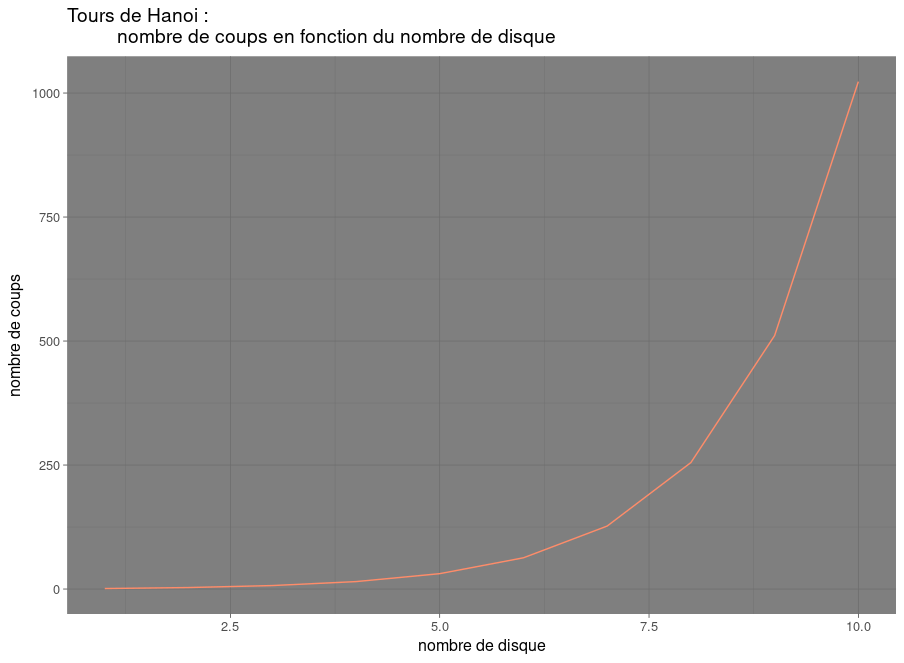
\includegraphics[scale=0.3]{graph_hanoi.png}
\end{frame}

%-------------------------------------------------------
%-------------------------------------------------------
\begin{frame}{Tours de Hanoï}{Première Implémentation}
%-------------------------------------------------------
  \begin{block}{Algorithme récursif:}
    Soit A, B, C les trois Tours. \\
    Déplaçons n disque de A vers C.
    \begin{itemize}
    \item Déplacer les $n-1$ plus petit de la tour A vers B
    \item Déplacer le plus gros disque de la tour A vers C
    \item Déplacer les $n-1$ disques de B vers C
    \end{itemize}
  \end{block}
\end{frame}


%-------------------------------------------------------
%-------------------------------------------------------
\begin{frame}{Tours de Hanoï}{Deuxième Implémentation}
%-------------------------------------------------------

\begin{block}{Problématique}
  Faire un affichage des tours et des disques. \\
  Tout en utilisant une représentation claire et efficace des données.

\end{block}
\end{frame}

\begin{frame}{Le Pavage de Penrose}
    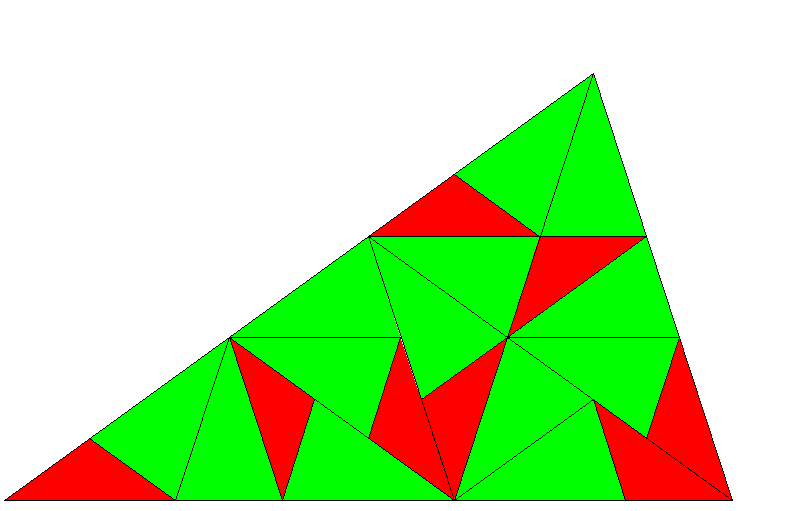
\includegraphics[scale=0.3]{penrose_example.png}
\end{frame}

\begin{frame}{Le Pavage de Penrose}{Principe de l'algorithme}
\begin{block}{Algorithme:}
  \begin{itemize}
    \item parcourir l'arbre des triangles;
    \item dessiner les triangle "feuilles" et leur contour.
  \end{itemize}
\end{block}
\begin{block}{Étapes nécessaires}
  \begin{itemize}
      \item Dessiner un triangle.
      \item Diviser un triangle.
      \item Dessiner le contour d'un triangle.
  \end{itemize}
\end{block}
\end{frame}

\begin{frame}{Le Pavage de Penrose}{Le dessin des contours}
  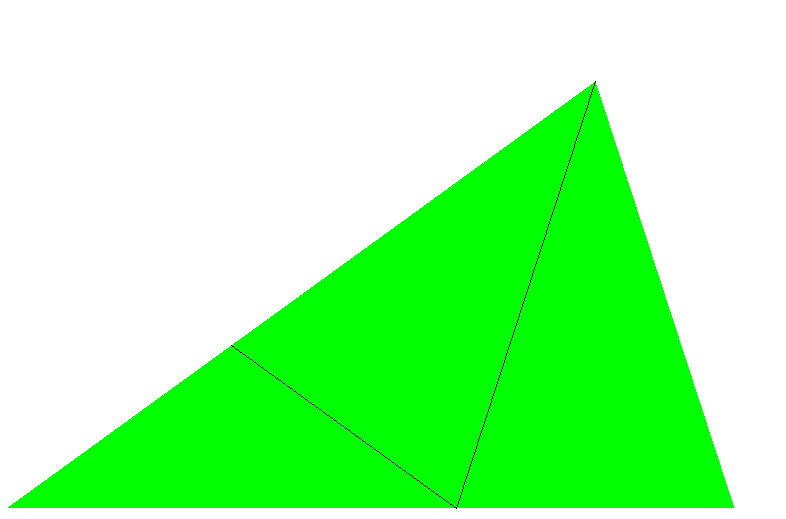
\includegraphics[scale=0.3]{penrose_inline1.png}
\end{frame}

\begin{frame}{Le Pavage de Penrose}{Le dessin des contours}
  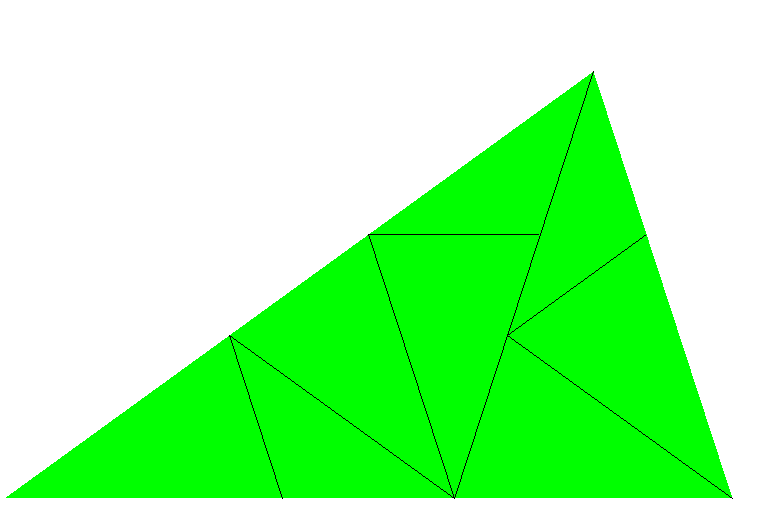
\includegraphics[scale=0.3]{penrose_inline2.png}
\end{frame}

\begin{frame}{Le Pavage de Penrose}{Animer le pavage}
  \begin{block}{Comment dessiner pas à pas ?}
    \begin{itemize}
        \item Parcours en largeur de l'arbre.
        \item À chaque profondeur, affichage des triangles.
        \item Affichage des contours.
    \end{itemize}
  \end{block}
\end{frame}

\begin{frame}{Le Pavage de Penrose}{Problèmes rencontrés}
  \begin{block}{Problème rencontrés:}
    \begin{itemize}
      \item coût en temps et en espace;
      \item complexification de la modularité.
    \end{itemize}
  \end{block}
\end{frame}
\end{document}
